\hypertarget{sos-s2} {
\section{Scrum of Scrums}\label{Scrum of Scrums} 
During this new sprint, the team had started on focus the console and develop 
games to proof the functionality of it, so, the team had created some Product 
Requirements Documents (PRD). One for the console and the others for TicTacToe 
and Pacman Games.
At the same time, during the Lead's Daily we discuss about the new change of 
the architecture, which present a change on the previous work of TicTacToe game. 
During this time, we also discuss to use Vulkan graphic API, so we have update 
the PRD for console to put it as new requirement.
}

\href{https://tree.taiga.io/project/joseluis-teran-coffeetime/wiki/fronted-team}{Link: TicTacToe and Pacman PRDs on Wiki Section - Taiga}.

\href{https://tree.taiga.io/project/joseluis-teran-coffeetime/wiki/backend-team}{Link: Console PRD on Wiki Section - Taiga}.

\href{https://github.com/Pending-Name-21/arquitecture/pull/5/files}{Link: Architecture Refactor - Pull Request on GitHub}.

\href{https://docs.vulkan.org/tutorial/latest/02_Development_environment.html#_linux}{Link: Vulkan Documentation}.

\href{https://tree.taiga.io/project/joseluis-teran-coffeetime/taskboard/sprint-2-12274}{Link: User Stories of Sprint 2 on Taiga}.

\begin{figure}
\centering
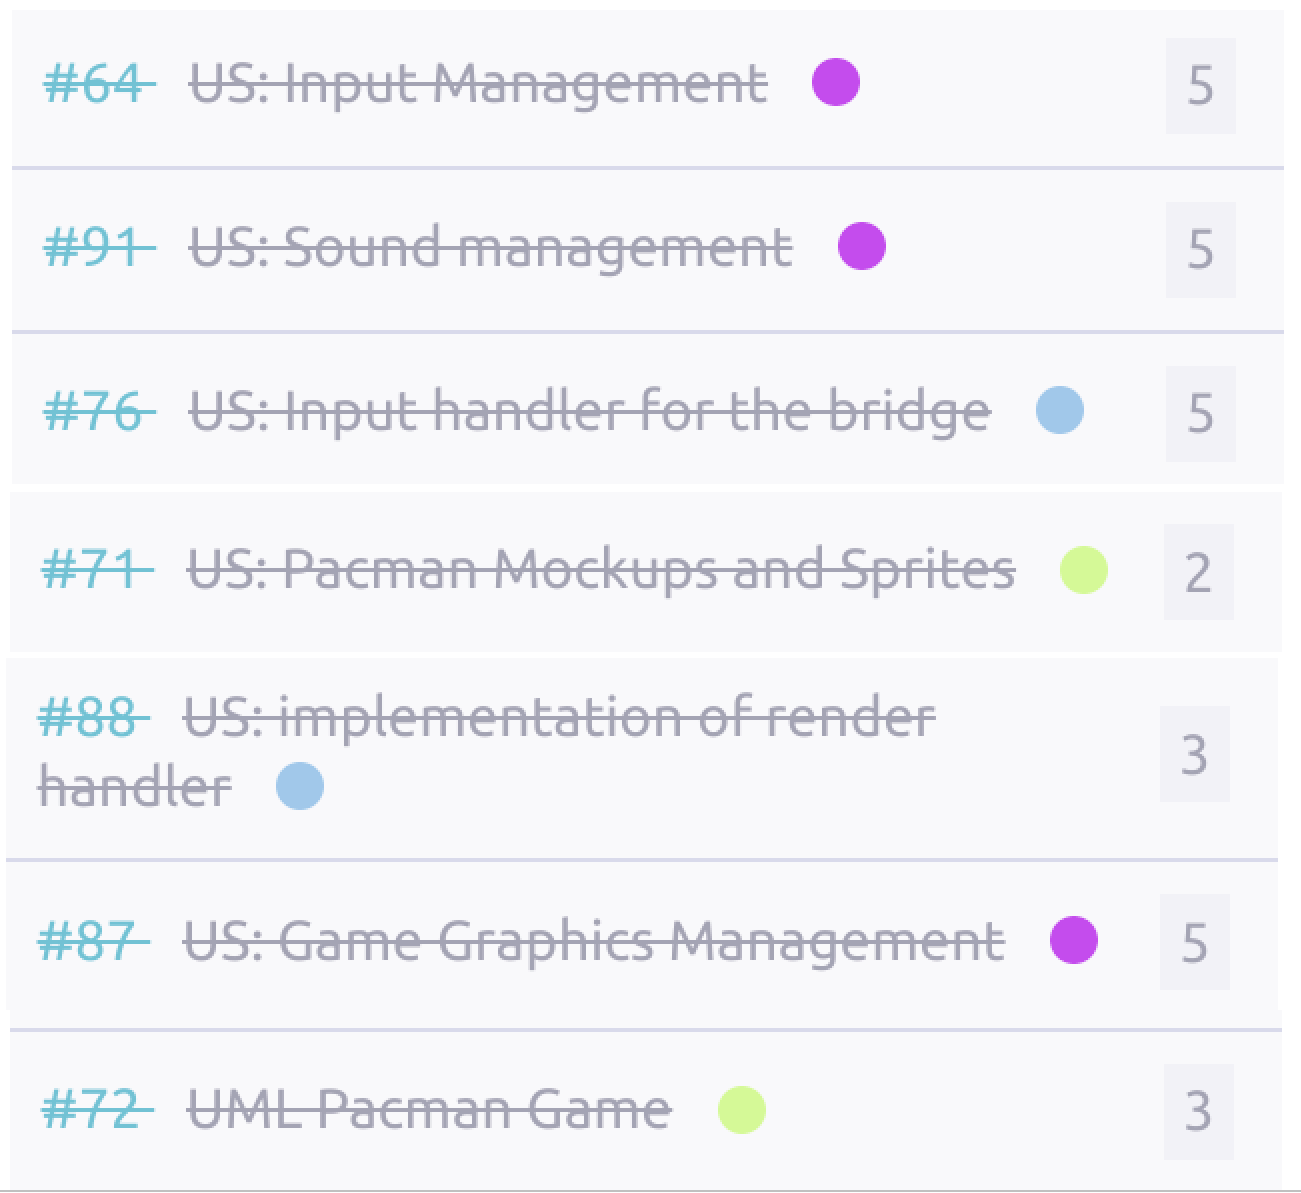
\includegraphics[width=8cm, height=15cm]{./assets/us-s2.png}
\end{figure}

\hypertarget{burndownchart-s2}{
\section{Burn Down Chart}\label{Burn Down Chart S2}}
\href{https://tree.taiga.io/project/joseluis-teran-coffeetime/taskboard/sprint-2-12274}{Link: Sprint 2 Board on Taiga}.

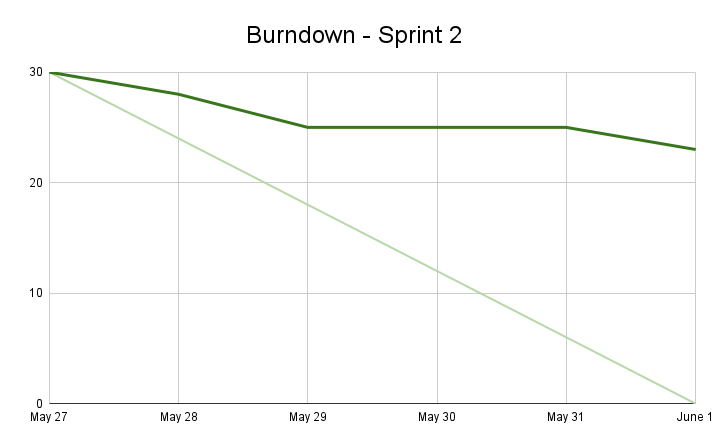
\includegraphics[width=\textwidth]{./artifacts/src/sprint-2/assets/Burndown-Sprint2.png}

\hypertarget{startstopcontinueactionitems-s2}{
\section{Start-Stop-Continue-Action Items}\label{Start-Stop-Continue-Action Items S2}}
\href{https://miro.com/app/board/uXjVKDO7l8M=/?moveToWidget=3458764590247693277&cot=14}{Link: Start-Stop-Continue-Action Items Sprint 2 on Miro}.

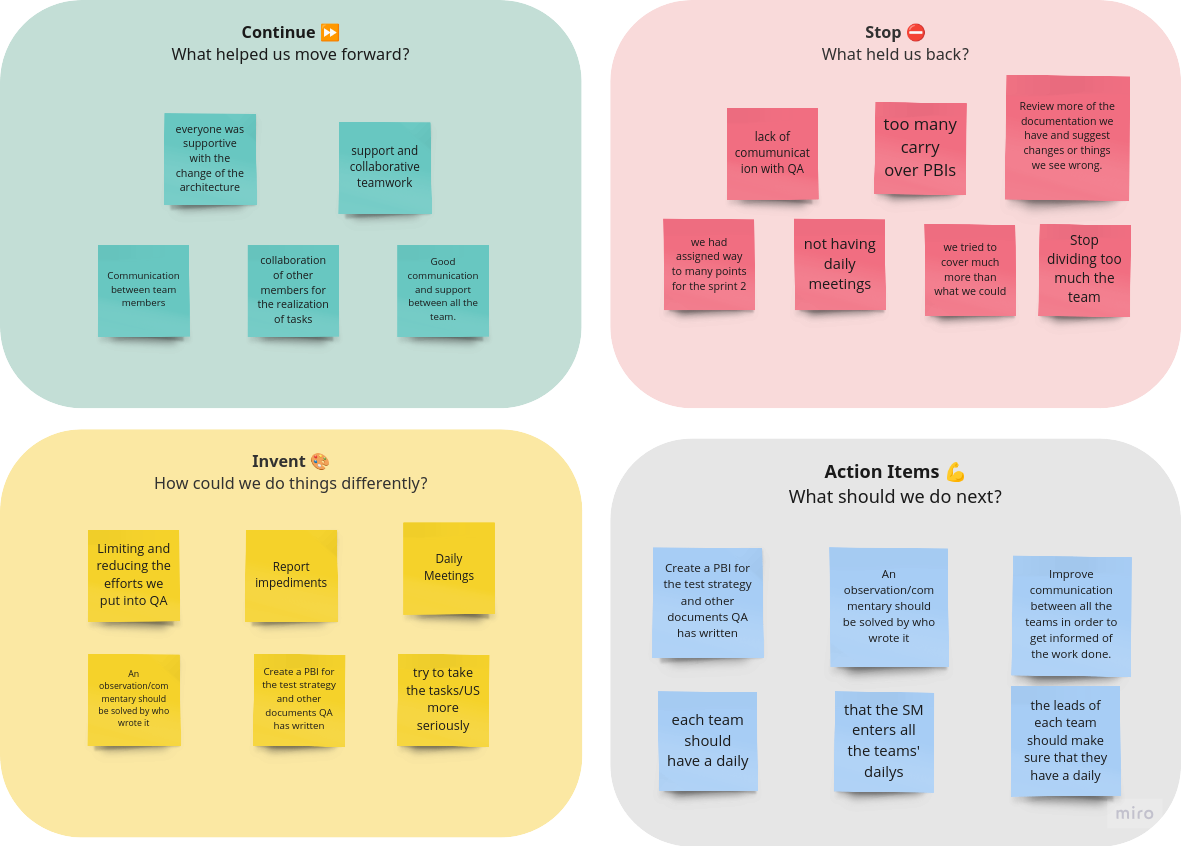
\includegraphics[width=\textwidth]{./artifacts/src/sprint-2/assets/retrospective-s2.png}

\end{document}
